\chapter{Design}

\section{Overall System Design}

\subsection{Short description of the main parts of the system}
\begin{itemize}
\item Home
This system will display the buttons required to  access the rest of the program and exit the program
\item Match
This system will display the details of a all the past matches that have been entered into the system. 
\item Player 
This system  will display all the details that have been entered by the user on an individual player.  
\item Team Sheet
This system will display the selected players in the selected formation, it will also have the substitutes listed to one side of the screen. The user will also be able to swap players in and out of the team sheet. Once the one user is happy with the team sheet they will be able to save it to the database for future reference. 
\item Goals
This system will display a list of goals from all past games that have been entered into the system, it will include bas details such as the scorer, the match it was scored in and the quantity.
\item Squad
This system will display a list of all the players in the squad.
\item Add Player
This system will ask for the user to input the basic details of a new player, such as name and position. These details will all be entered into text boxes.
\item Add Goals
This system will ask for the user to select the match and goal scorer from a drop down menu, The user will then have to enter the quantity scored by the selected player in the selected game. 
\item Add Match
This system will ask for the user to input the basic details of a recent match, such as the result and the opposition.

\end{itemize}
\section{User Interface Designs}
\begin{figure}[H]
	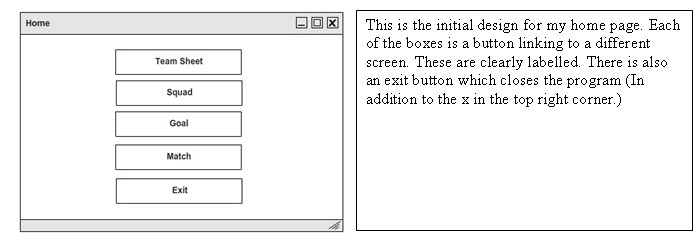
\includegraphics{HomeUifTxt}
	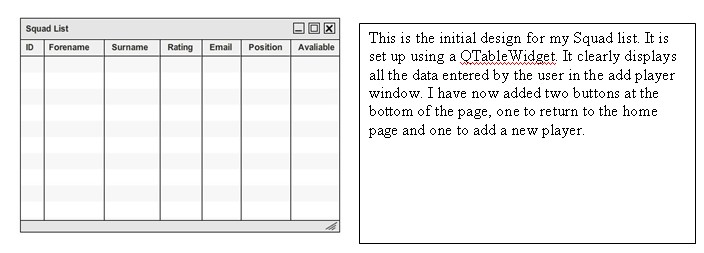
\includegraphics{SquadListUifTxt}
	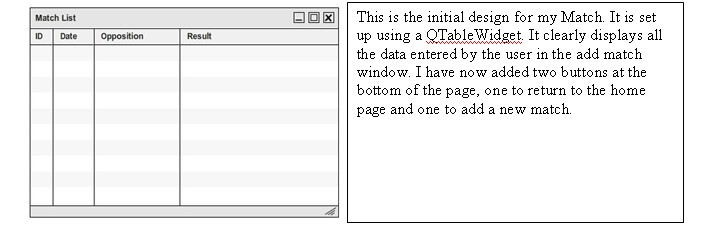
\includegraphics{MatchListUifTxt}
	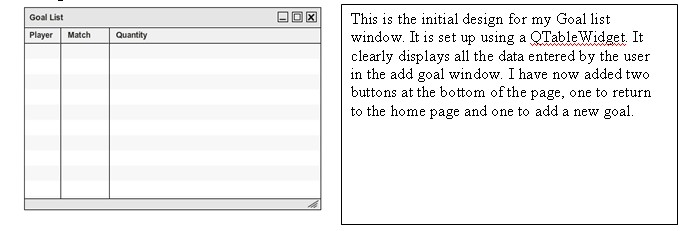
\includegraphics{GoalListUifTxt}
	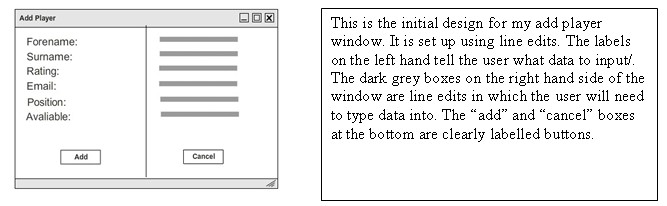
\includegraphics{addPlayerUifTxt}
	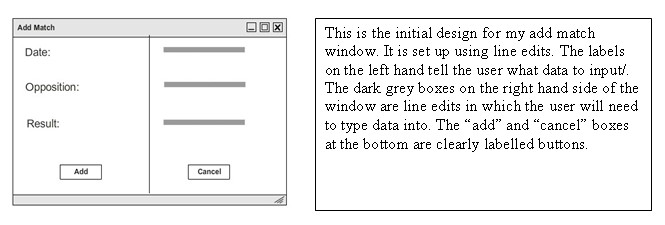
\includegraphics{addMatchUifTxt}
	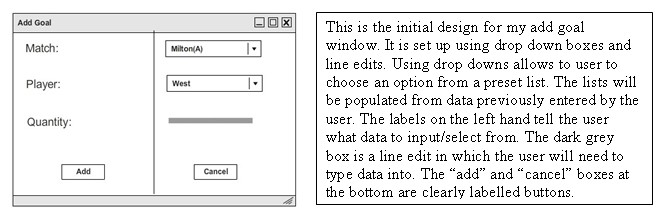
\includegraphics{addGoalUifTxt}
\end{figure}
\section{Hardware Specification}
The system will need to run on a desktop computer, a laptop and on a tablet. It will need to run on the computers at 1360x768, in a 16:9 aspect ratio screen as well the IPad's 1024x768-pixel display, in a 4:3 aspect ratio. A keyboard will be needed for input as well as a pointer device to navigate around the system. A display will be used for the output of the program. The data for the program will be held on a hard drive.
\section{Program Structure}

\subsection{Top-down design structure charts}

\subsection{Algorithms in pseudo-code for each data transformation process}

\subsection{Object Diagrams}

\subsection{Class Definitions}
\begin{figure}[H]
	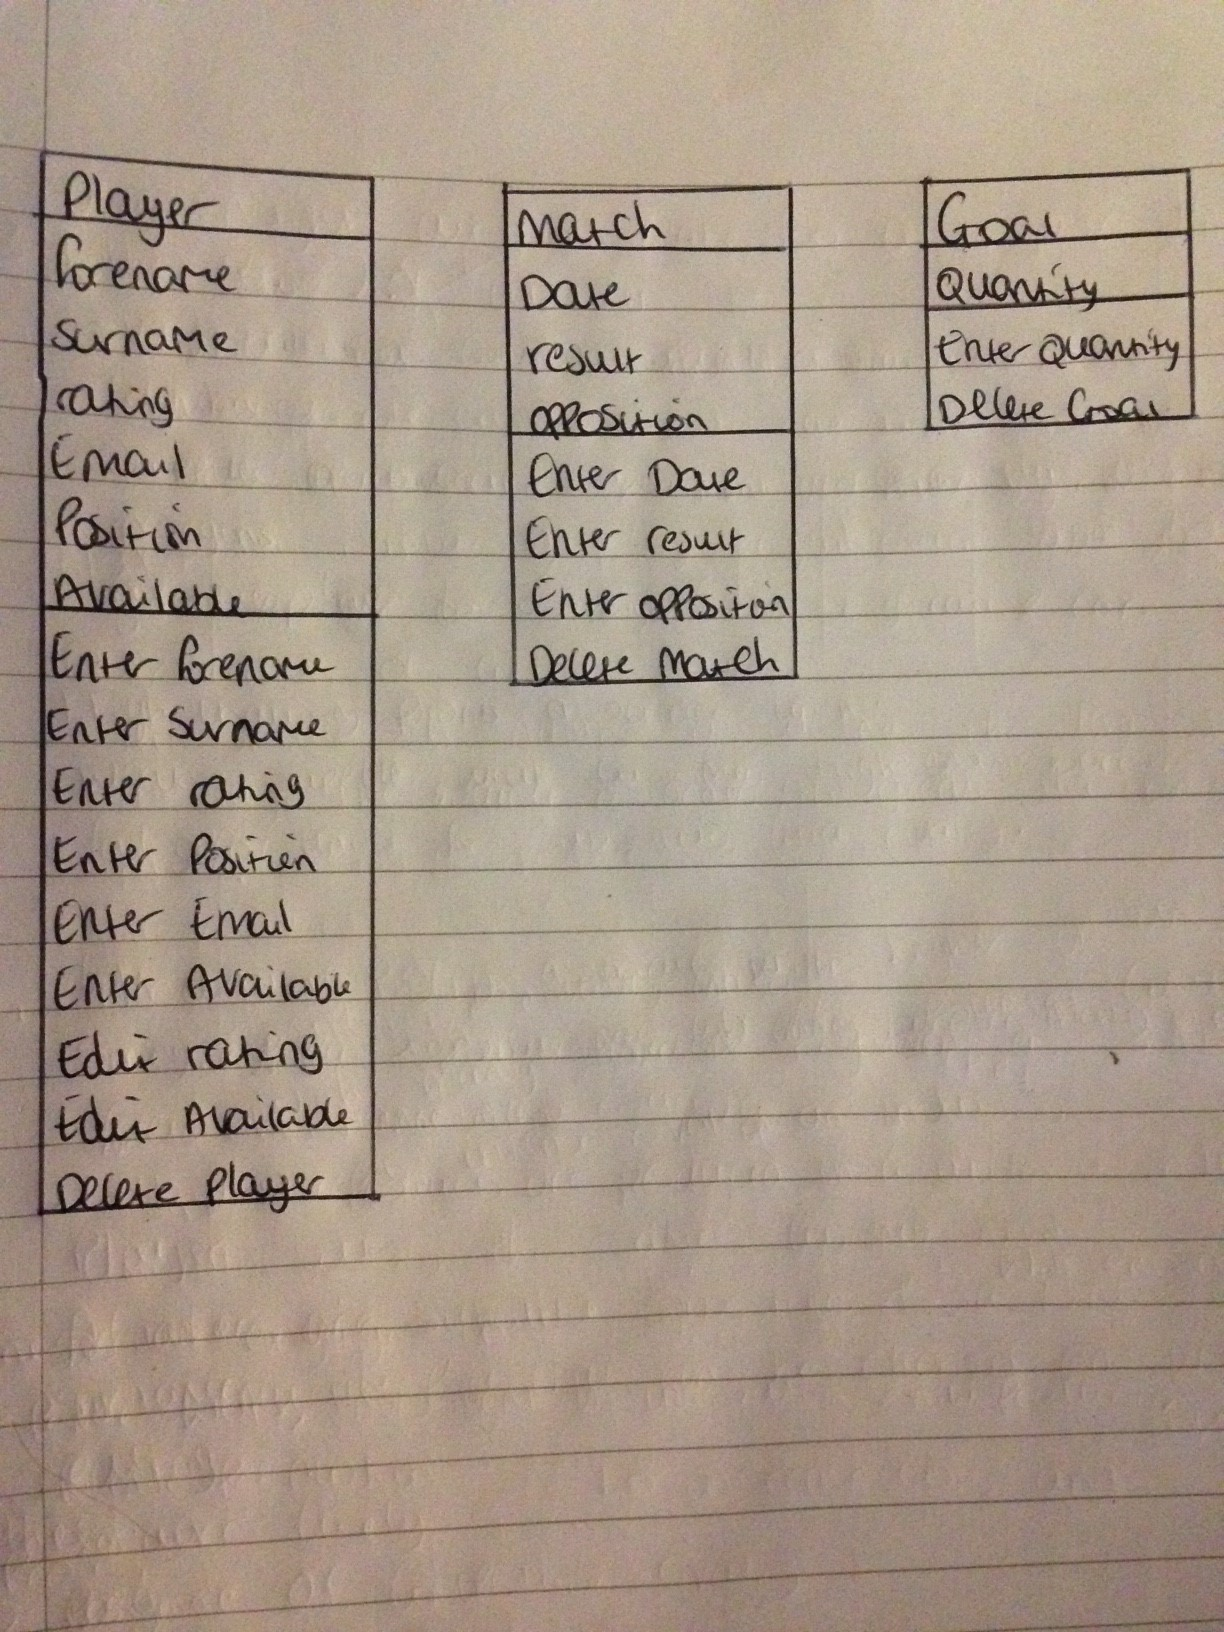
\includegraphics[width=150mm]{classdef}
\end{figure}

\section{Prototyping}

\section{Definition of Data Requirements}

\subsection{Identification of all data input items}
\begin{itemize}
\item Player first name
\item Player second name
\item Player rating
\item Player email
\item Player position
\item Player availability
\item Match Date
\item Match opposition
\item Match result
\item Goal Quantity 

\end{itemize}

\subsection{Identification of all data output items}
\begin{itemize}
\item team sheet
\item New goal
\item Goal table
\item Player table
\item Match table
\end{itemize}
\subsection{Explanation of how data output items are generated}
\begin{itemize}
\item The team sheet will be generated by the user selecting players from the player table. The player data will have been previously entered by the user and stored in a global database. To select the players, the player table will need to be used. Again the data in this table will come from the global database.  
\item The new goal will display data in drop down boxes for the user to select from. This will be data that the user has previously entered into the system. It will be stored in a global database. 
\item The goal table will be generated by taking the data that the user has previously input, now stored in a global database and displaying it in a table format for the user to see. The user will also be given the option to add more data to the table.
\item The Player table will display all the player details from the "new player" window. The data will be user entered and stored in a global database.
\item The match table will generate its data from the global database. The data will be put in columns so that it is easily readable to the user. The data will have been previously entered by the user based on the recent match that had been played.  
\end{itemize}

\subsection{Data Dictionary}
\begin{table}[H]
\centering
%\begin{tabular}{|p{2.5cm}|p{1cm}|p{1.5cm}|p{2.5cm}|p{2.5cm}|p{2.5cm}|} 
\begin{tabular}{|l|l|l|l|l|l|} 
\hline
Name            & Data Type & Length   & Validation                    & Example Data    & Comment                        \\ \hline
PlayerID        & Integer   & 3 Digits & 3 Digits, Must exist          & 123             & Unique to each player          \\ \hline
PlayerForename  & String    & 15 Chars & Minimum of 3 digits           & Harry           & First name, capital first char \\ \hline
PlayerSurname   & String    & 20 Chars & Minimum of 3 digits           & West            & Surname, capital first char    \\ \hline
PlayerPosition  & String    & 2 Chars  & Must be 2 chars               & GK              & In caps                        \\ \hline
PlayerRating    & Integer   & 2 Digits & Maximum of 2 digits           & 8               & Most likely to only be 1 digit \\ \hline
PlayerEmail     & String    & 50 Chars & Must have an @                & Hwest@gmail.com & Contact for the player         \\ \hline
MatchID         & Integer   & 3 Digits & 3 digits, must exist          & 869             & Unique to match                \\ \hline
MatchDate       & String    & 8 Chars  & Must exist                    & 23/09/14        & Date of the match              \\ \hline
MatchResult     & String    & 1 Chars  & Must exist                    & W               & W=Win, L=lose, D=Draw          \\ \hline
MatchOpposition & String    & 20 Chars & Minimum of 3 digits           & Milton          & Opposition name                \\ \hline
GoalQuantity    & Integer   & 2 Digits & At least one digit must exist & 2               & 99\% will only be one digit    \\ \hline
\end{tabular}
\end{table}
\subsection{Identification of appropriate storage media}
Because my system will only need to be accessed by one computer and one portable device the database file can be stored on a hard drive and copied across when required. If the client chooses to use the system on a portable device  they would need to transfer the database file across. No data would need to be added/deleted from the portable device. This would all be done from the main computer. therefore the files would never need transferring back to the main computer from the portable device. This means the files on the portable device would only need to be readable. The client has no personal server for which the files can be stored on. Therefore the database file will need to be easily accessible on the main computers hard drive so that the user can easily copy them across to the portable device when they are needed. 
\section{Database Design}

\subsection{Normalisation}

\subsubsection{ER Diagrams}
\begin{figure}[H]
	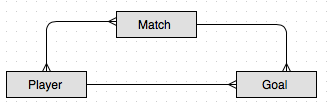
\includegraphics{ER}
\end{figure}

\subsubsection{Entity Descriptions}
Player( {\ul PlayerID},PlayerForename,PlayerSurname,PlayerRating,PlayerEmail,PlayerPosition,PlayerAvailable)
Match({\ul MatchID},MatchDate,MatchResult,MatchOpposition)
Goals(MatchID,PlayerID,GoalQuantity)
\subsubsection{1NF to 3NF}

\subsection{SQL Queries}
\begin{table}[]
	\centering
	\caption{My caption}
	\label{my-label}
	\begin{tabular}{ll}
		SQL Statement                                                                                                                                                                                                                      & Description                                                                                                                                                                                                                               \\
		\begin{tabular}[c]{@{}l@{}}"""create table if not exists Player,\\ (PlayerID integer,\\ forename text,\\ surname text,\\ rating integer,\\ email text,\\ position text,\\ available text,\\ primary Key(PlayerID))"""\end{tabular} & This is an example of an SQL statement that creates a new table called Player, with the attributes Forename, Surname, Rating, Email, Position and Available. The primary key is set to PlayerID.                                          \\
		"insert into Goal(GoalID,opposition,forename,quantity) values ((SELECT max(GoalID) FROM Goal)+1,'\{0\}', '\{1\}', '\{2\}')".format(opposition,forename,quantity)                                                                   & This is an example of an SQL statement to add records to the database. In this case, it is entering a new goal record with the attributes opposition, forename,quantity. The GoalID attribute is being generated in the SELECT statement. \\
		SELECT max(GoalID) FROM Goal)+1                                                                                                                                                                                                    & This is an example of an SQL statement that generates an ID, it selects the max from a field in a record and adds 1 to it. This is used within the entering of a record into the database.                                               
	\end{tabular}
\end{table}
\section{Security and Integrity of the System and Data}
There is a very limited amount of data on the system that needs to be secure. This is the email addresses. The program will only be handed out to certain individuals on wont be available for on line download. The people that are handed the software are authorized to see the data. If they wish to install the data on a shared computer, e.g a home pc, then the data does not need protecting as it will be available on the email application that the client uses. Therefore no extra personal data is being stored with in the system. The data will also be entered by an authorized user and therefore will have already been seen. 

\subsection{Security and Integrity of Data}
There is a very limited amount of data on the system that needs to be secure. This is the email addresses. The program will only be handed out to certain individuals on wont be available for on line download. The people that are handed the software are authorized to see the data. The system will require a password when it is booted up. This means that only authorized individuals can access the system.  

\subsection{System Security}
The system will have a password entry to stop any unauthorized users entering the system. This protects the email addresses stored on the system. If the system wasnt secure then the system would be prone to these email addresses being stolen, This would be breach the data protection act 1998. 
\section{Validation}

\section{Testing}

